\chapter{SparkSQL}

\section{Relational Algebra}	
	\subsection{Operators}
		\par
		Relational algebra operators are a operations on data that fit well the relational algebra model.
		\newline
		In traditional RDBMS, queries involve retrieval of small amounts of data while now we should keep in mind the workload underlying MapReduce: full scans of large amounts of data and queries that process all data (not selective\footnote{This is true in general. Most ETL jobs (Extract Transform Load) involve selection and projection to do data preparation.}).
		\newline
		Relations\footnote{A relation is a table.} (however big) can be stored in a distributed file system, if they don't fit in a single machine, they're broken into pieces.
		\subsubsection{Selection $\sigma_C(R)$}
			\par
			Apply a condition \textit{C} to each tuple of relation \textit{R}.
			\newline
			Produce in output a relation containing only tuples for the attributes\footnote{Attributes are the column headers of the table.} in \textit{S}.
		\subsubsection{Projection $\pi_S(R)$}
			\par
			Given a subset \textit{S} of attributes of a relation R, produce in output a relation containing only tuples for the attributes in \textit{S}.
		\subsubsection{Union, Intersection and Difference}
			\par
			Well known operators on sets, applied to the sets of tuples in two relations that have the same schema\footnote{The set of attributes $A_1, A_2, ..., A_n$ of a relation $R(A_1, A_2, ..., A_n)$ is called a schema.}.
		\subsubsection{Natural Join $R \bowtie S$}
			\par
			Given two relations, compare each pair of tuples, one for each relation. If the tuples agree on all the attributes common to both schema, then produce an output tuple that has components on each attribute, otherwise produce nothing.
			\newline
			The join condition can be on a subset of attributes.
		\subsubsection{Grouping and Aggregation $\gamma_X(R)$}
			\par
			Given a relation \textit{R}, partition its tuples according to their values in one set of attributes \textit{G} (grouping attributes). For each group, aggregate the values according to aggregation functions (SUM, COUNT, AVG, MIN, MAX) over other attributes.
			\newline
			\textit{X} is a list of elements that can be a grouping attribute or an expression $\theta(A)$, where $\theta$ is an aggregation function and \textit{A} is an attribute NOT among the grouping attributes.
			\newline
			The result is a relation with a tuple for each group. That tuple has a component for each of the grouping attributes with the common value of the tuples in that group, and another component for each aggregation function, with the aggregate value for that group\footnote{The COUNT function does not consider the values of an attribute, it just count the number of tuples. In SQL there is a COUNT DISTINCT operator to count the number of different values.}.
			
	\subsection{Operators and MapReduce}
		\subsubsection{Selection}
			\par
			Selection can be implemented in the map phase alone (but also in the reduce portion).
			\newline
			During the map phase, for each tuple \textit{t} in \textit{R}, check if \textit{t} satisfies the condition \textit{C}, if so, emit a key/value pair \textit{(t, t)}\footnote{There is no use for the second \textit{t}, it could be a 1 for a better implementation.}.
			\newline
			Then, use an identity reducer. We can't choose the number of mappers but we can choose the number of reducers, it is a matter of degree of parallelism. We can use a single reducer because it is a simple task, but if the reducer is loose (it makes a lot of pairs pass) then all of the pairs are going to hit just one machine so it is better to have multiple reducers.
			\newline
			The output is not exactly a relation because it does not have the same schema as the input.
		\subsubsection{Projection}
			\par
			In the map phase, for each tuple \textit{t} in \textit{R}, construct a tuple \textit{t'} by eliminating those components whose attributes are not in \textit{S}. Emit a key-value pair \textit{(t', t')}.
			\newline
			The reduce operation is duplicate elimination. For each key \textit{t'} produced by any of the map tasks, fetch \textit{t', [t', ..., t']} and emit a key-value pair \textit{(t', t')}.
			\newline
			The reducer operation is associative and commutative, so it is possible to optimize MapReduce by using a combiner in each mapper.
		\subsubsection{Union}
			\par
			Suppose the relations \textit{R} and \textit{S} have the same schema, the mappers don't do much, for each tuple \textit{t} in \textit{R} or \textit{S}, they emit a key-value pair \textit{(t, t)}.
			\newline
			Reducers do duplicate elimination, for each key \textit{t} there will be either one or two values, they emit \textit{(t, t)} in either case.
		\subsubsection{Intersection}
			\par
			Suppose the relations \textit{R} ans \textit{S} have the same schema, the map function is the same as for union, an identity mapper. During the reduce phase, if the key \textit{t} as value list \textit{[t, t]} (the key has been found two times), then emit the key-value pair \textit{(t, t)}, otherwise, emit \textit{(t, NULL)}.
		\subsubsection{Difference}
			\par
			Assume the relations \textit{R} and \textit{S} have the same schema, the only way a tuple \textit{t} can appear in the putput is if it is in \textit{R} but not in \textit{S}. The map function passes tuples from \textit{R} and \textit{S} to the reducer but it must also pass information about where the tuple came from.
			\newline
			In the map phase, emit tuples \textit{(t, 'R')} or \textit{(t, 'S')}.
			\newline
			In the reduce phase, for each key \textit{t}, if it is associated to \textit{'R'}, emit \textit{(t, t)}. Otherwise (it is associated to \textit{['R', 'S'], ['S', 'R'] or 'S'}), emit the key-value pair \textit{(t, NULL)}.
		\subsubsection{Join}
			\par
			Suppose we have two relations \textit{R(A, B)} and \textit{S(B, C)}, we must find tuples that agree on their \textit{B} components. We shall use the \textit{B-value} as the key, the value will be the other component and the name of the relation, so that the reducer knows from which relation each tuple is coming from.
			\newline
			In the map phase, for each tuple \textit{(a, b)} or \textit{(b, c)} emit the key-value pair \textit{(b, ('R', a))} or \textit{(b, ('S', c))}.
			\newline
			In the reduce phase, each key \textit{b} will be associated to a list of pairs that are either \textit{('R', a)} or \textit{('S', c)}. Emit pairs of the form $(b, [(a_1, b, c_1), (a_2, b, c_2), ..., (a_n, b, c_n)])$.
			\newline
			In general, for \textit{n} tuples in relation \textit{R} and \textit{m} tuples in relation \textit{S}, all with a common \textit{B-value}, we end up with \textit{nm} tuples in the result. Therefore if all tuples of both relations have the same \textit{B-value}, then we're computing the Cartesian product.
		\subsubsection{Grouping and Aggregation}
			\par
			Let \textit{R(A, B, C)} be a relation to which we apply $\gamma_{A, \theta(B)}(R)$, under the simplifying assumption of using one grouping attribute and one aggregation function, we know that: the map operation prepares the grouping, that is done by the framework, and the reducers compute the aggregation.
			\newline
			In the map phase, for each tuple \textit{(a, b, c)} emit the key/value pair \textit{(a, b)}.
			\newline
			In the reduce phase, each key represents a group, apply $\theta$ to the list $[b_1, b_2, ..., b_n]$ and emit the key-value pair \textit{(a, x)} where $x = \theta([b_1, b_1, ..., b_n])$.
	
\section{DataSource and DataFrame API}
	\par
	The DataSource API is used to \textbf{read and write from a variety of formats, either built-in or external}.
	\newline
	It has a unified interface: the functions read, load, write and save create new \textbf{I/O builders}. The builder methods are used to specify the data format, define data partitioning, handle existing data and more.
	\newline
	\par
	The idea of Dataframe is borrowed from Python Pandas: \textbf{tabular data with an API}. They are an abstraction for selecting, filtering, aggregating and plotting structured data.
	\newline
	The schema is applied only on read, not on write as traditional DBMS. Schema inference can be automatic, it is a distributed collection of rows organized into named columns.
	\newline
	The Dataframe \textbf{introduces structure to the data of the low-level RDD} and it specifies relational operators (select, join, aggregate, filter).
	\begin{figure}[H]
		\centering
		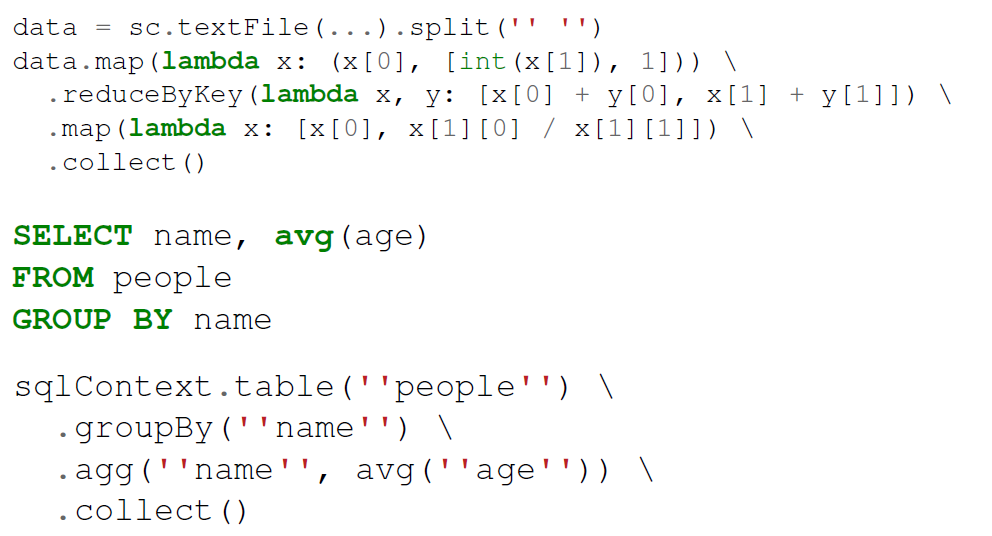
\includegraphics[width=0.8\linewidth]{images/dataframe.png}
		\caption{\textit{Comparison between RDDs, SQL and Dataframes.}}
	\end{figure}

\section{SparkSQL Architecture}
	SparkSQL borrows many ideas from traditional RDBMSs, it does optimization for efficiency and performance (logical plan and physical plan) using a sophisticated cost model (cost based or rule based).
	\begin{figure}[H]
		\centering
		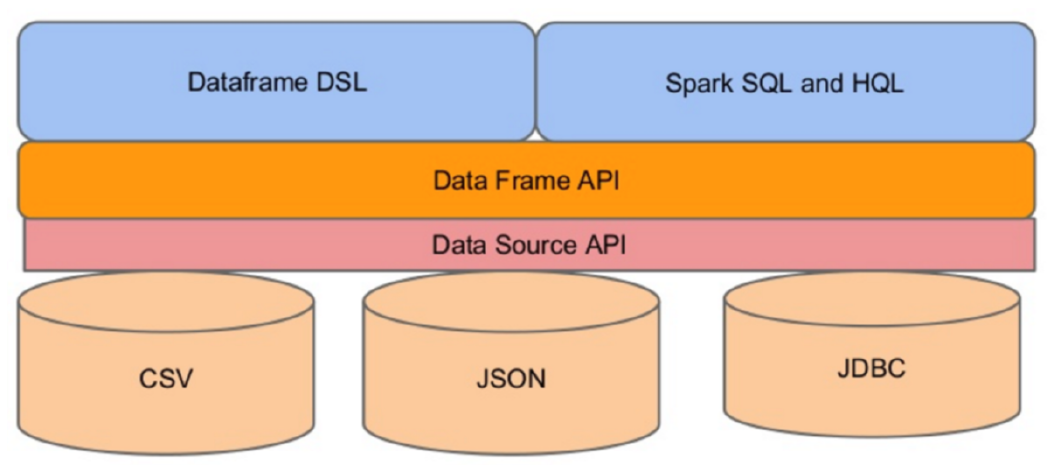
\includegraphics[width=0.8\linewidth]{images/sparksqlarch.png}
		\caption{\textit{Global view of SparkSQL architecture.}}
	\end{figure}
	The SparkSQLContext goes through a series of steps to get the data.\newline
	First, it builds an unresolved logical plan using the DataFrame and the SQL Abstract Syntax Tree. The AST then take information from a Catalog (e.g the name of attributes to reference the data) to produce a more human readable plan.\newline
	The logical plan (or tree) is optimized moving operators around, it defines the \textbf{logical flow of data from the extraction to the end}.\newline
	\begin{figure}[H]
		\centering
		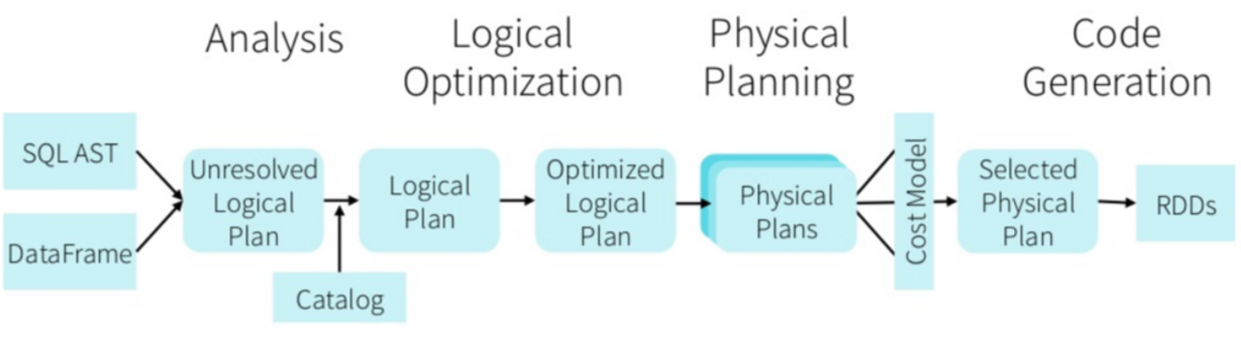
\includegraphics[width=0.8\linewidth]{images/sparksqlcontext.png}
		\caption{\textit{Flow of data through the SparkSQLContext.}}
	\end{figure}
	From the optimized logical plan a list is made of all the possible physical plans, these are then evaluated by a cost model which is continuously refined: it associates a cost to the operators and the cardinality.\newline
	Finally the selected physical plan is translated in Java ByteCode that will be submitted to the cluster.\newline
	\newline
	The \textbf{Catalyst optimizer} is the component taking care of these steps. It exploits some scala language features like \textit{Quasiquotes} for better tree manipulation.\newline
	\newline
	The \textit{project Tungsten} is a valid alternative that better exploits modern compilers, CPUs and cache locality. The more important feature is manages memory explicitly and eliminates the overhead of JVM object model and garbage collection.
	
